\chapter{Modelo de elementos finitos para una fibra elastica 1D}
\label{cap1}


\section{Objetivos de la práctica}
\label{sec:objetivos}

En esta práctica se ejemplifica la programación en \texttt{Matlab} de un código, basado en la técnica de los elementos finitos, capaz de resolver un problema elástico en una dimensión en el que se carga una fibra de un material biológico. Partimos de las siguientes premisas:
\begin{enumerate}
	\item
	Se han dado en la clase teórica, y aparecen a su vez en este documento, una serie de nociones teóricas en cuanto a la construcción de matrices de rigidez elementales, las cuales han de ser programadas por el alumnado.
	\item
	A su vez, estas matrices elementales han de pasar a formar parte de un sistema global a través del ensamblado de la matriz de rigidez global, para la cual también se han explicado unas nociones teóricas.
	\item
	Para la resolución del sistema de ecuaciones es necesario conocer las condiciones de contorno de carga y desplazamiento del problema. Se han de aplicar las mismas al sistema matricial que se ha desarrollado en \texttt{Matlab}.
	\item
	El sistema puede ser resuelto finalmente, y, con los resultados obtenidos, se puede comparar con solución analítica que el propio alumno ha de deducir y calcular en \texttt{Matlab}. Dicha comparación ha de ser llevada a cabo con las herramientas de dibujo de \texttt{Matlab}.
\end{enumerate}
Esta pr\'actica permite a los alumnos conocer como es un código de Elementos Finitos de forma simplificada. La pr\'actica 8.2 es una continuación de los contenidos te\'oricos de esta, si bien la 8.2 ahonda en la resoluci\'on con un software de terceros: \texttt{FeBio}. Servirá tambien el resultado obtenido con dicho software para la comparaci\'on con el desarrollado en esta pr\'actica 8.1.

\section{Base teórica}
\label{sec:teoria}

%\subsection{Governing equations}
\subsection{Ecuaciones de gobierno}

La ecuación que gobierna el fenómeno físico es la de una fibra elástica cuyo  desplazamiento se define por \(u(x)\). Como se ha descrito, esta es una ecuación elíptica lineal en una dimensión, con la siguiente forma:
\begin{equation}\label{eq:gov}
\frac{\mathrm{d \sigma}}{\mathrm{d} x} + q(x)
=\frac{\mathrm{d}}{\mathrm{d} x}\left(E A \frac{\mathrm{d} u}{\mathrm{d} x}\right)+q(x)=0
\end{equation}
donde  $E$ es el módulo de Young, un parámetro elástico del material que describe su rigidez y $A$ su \'area. $q(x)$ representa las fuerzas volumétricas para este problema, por unidad de longitud. La resolución numérica de este problema supone encontrar un \(u(x)\), en el intervalo abierto $(0,L)$, tal que el sistema esté en equilibrio teniendo en cuenta unas condiciones de contorno definidas para el problema en cuesti\'on.

\subsection{Condiciones de cortorno y fuerzas volumétricas}

Las posibles condiciones de contorno que nos encontramos en el problema a resolver se resumen en la Fig.~\ref{fig:CC1D}.

\begin{figure}[!htp]
\centering
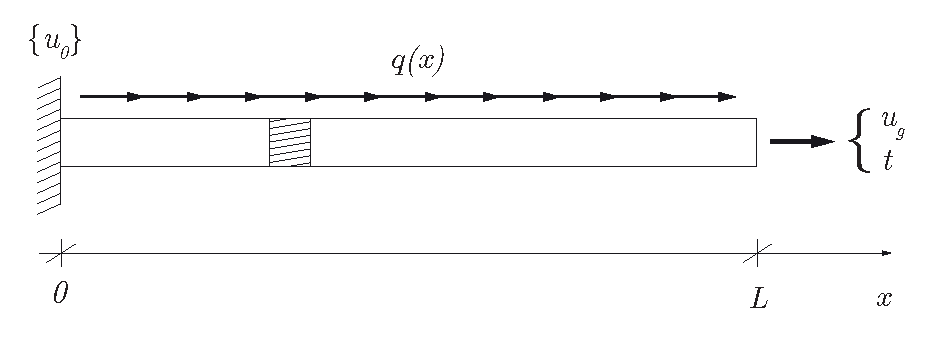
\includegraphics[width=0.8\textwidth]{figuras_1/1D.pdf}
\caption{Definición del problema y sus condiciones de contorno.}
\label{fig:CC1D}
\end{figure}

Sobre las condiciones de contorno, nos podemos encontrar de dos tipos:
\begin{itemize}
\item \textit{Tipo Dirichlet o Esenciales}\\
Aquellas que se aplican en el campo en el que hemos definido la ecuación diferencial, en nuestro caso \(u(x)\). En este caso son condiciones de contorno ``en desplazamiento''.
$$
u(0)=u_0
$$$$
u(L)=u_g
$$
\item \textit{Tipo Neumann o Naturales}\\
Aquellas que se aplican en la derivada espacial del campo en el que hemos definido la ecuación diferencial, que teniendo en cuenta la ecuación constitutiva, sería:
$$
t= E \frac{\mathrm{d} u}{\mathrm{d} x} \biggr\rvert_{x=L}
$$
Estas podrían considerarse como condiciones de contorno ``en fuerzas''.
\end{itemize}

Por otro lado nos encontramos las \textit{fuerzas volumétricas} o  \textit{distribu\'idas}, aquellas que se aplican a todo el dominio y que en la ecuación~\eqref{eq:gov} están definidas por $q(x)$. Estas fuerzas pueden depender de la posición o bien ser constantes.

Un ejemplo de este tipo de fuerzas en el problema mecánico son aquellas asociadas a la gravedad, las cuales dependen de una secci\'on $A(x)$, dependiente o no de la posici\'on, y una densidad, que tambi\'en puede variar a lo largo del dominio, por lo que dicha fuerza tambi\'en variaría con la posición:
$$
q(x) = A(x) \rho(x) g
$$

En el ejemplo a resolver en esta práctica, $q(x)$ será una función dada dependiente de la posición, representando así la carga aplicada por unidad de longitud.

\clearpage
\section{Disctretización de las ecuaciones de gobierno}
\label{sec:disc}

\subsection{Formulación fuerte y solución analítica}
\label{sec:analitica}
La ecuación \eqref{eq:gov} se puede considerar como la formulación fuerte del problema, que se denomina así porque se obliga a que la ecuación en derivadas parciales se cumpla en cada punto del intervalo de interés, $(0,L)$. 

Como vemos, dicha ecuación involucra una derivada segunda del campo \(u(x)\), lo que implica que dicho campo ha de ser derivable dos veces con respecto a x.\\

A continuación se detalla la obtención de la solución analítica. Partimos de la integración de la formulación fuerte entre un punto $y\in(0,L)$ y L:
\begin{eqnarray}
A \int_y^L \frac{\mathrm{d \sigma}}{\mathrm{d} x} \mathrm{d} x &=& -\int_y^L  q(x) \mathrm{d} x \\
\sigma(L)-\sigma(y) &=& -\frac{1}{A}\int_y^L  q(x) \mathrm{d} x 
\end{eqnarray}
Si empleamos la definición que nos aporta la ecuación constitutiva, $\sigma = E u_{,x}$:
\begin{equation}
E \frac{\mathrm{d} u(y)}{\mathrm{d} y} = E \frac{\mathrm{d} u}{\mathrm{d} x} \biggr\rvert_{x=L}  +\frac{1}{A}\int_y^L  q(x) \mathrm{d} x 
\end{equation}
De nuevo, integramos entre 0 y un punto $z\in(0,L)$:
\begin{equation}
\int_0^z E \frac{\mathrm{d} u(y)}{\mathrm{d} y} \mathrm{d} y = \int_0^z \left( E \frac{\mathrm{d} u}{\mathrm{d} x} \biggr\rvert_{x=L}  +\frac{1}{A}\int_y^L  q(x) \mathrm{d} x \right) \mathrm{d} y
\end{equation}
Asumiendo que $E$ es constante, al que la derivada de $u$ con respecto a $x$ en el punto $x=L$, el resultado obtenido de la integral es:
\begin{equation}
E u(z) - E u(0) = E \frac{\mathrm{d} u}{\mathrm{d} x} \biggr\rvert_{x=L} z + \frac{1}{A}\int_0^z\int_y^L  q(x) \mathrm{d} x \mathrm{d} y
\end{equation}
Por tanto, la solución de $u(z)$ resulta:
\begin{equation}\label{eq:anal}
u(z)  = u(0) +  \frac{\mathrm{d} u}{\mathrm{d} x} \biggr\rvert_{x=L} z  +\frac{1}{EA}\int_0^z\int_y^L  q(x) \mathrm{d} x \mathrm{d} y
\end{equation}
La solución analítica de la ecuación~\eqref{eq:anal} depende de dos constantes para las que son necesarias la aplicación de las dos condiciones de contorno que tengo, $u(0) $ y $\frac{\mathrm{d} u}{\mathrm{d} x} \biggr\rvert_{x=L}$, condiciones de contorno esencial y natural respectivamente. Para el caso de no tener una condición de contorno natural en el extremo $x=L$ sino una condición en desplazamientos, el término $\frac{\mathrm{d} u}{\mathrm{d} x} \biggr\rvert_{x=L}$ se puede calcular imponiendo $z=L$, siendo que $u(L)$ es conocido.

Para el caso particular en que las condiciones de contorno sean: $u(0) = 0$ (extremo fijo) y $EA\mathrm{d}u/\mathrm{d}x|L = P$ (carga $P$ en $x = L$), y la fuerza distribuida sea una función lineal $q(x) = q0+rx$, se desea obtener la expresión de la solución analítica. \textbf{Dicha resolución ha de ser realizada por los alumnos.}

Teniendo en cuenta las hipótesis realizadas, solo podremos obtener expresiones analíticas para valores sencillos de $E(x)$ y $f(x)$, abandonando la idea cuando estos valores se complican, por lo que hemos de buscar soluciones aproximadas. Una de las técnicas más empleadas es la del método de los elementos finitos, para el que necesitamos la forma débil del problema, que pasamos a describir en la siguiente sección.

\subsection{Formulación débil}
\label{sec:debil}

Esta formulación se consigue con una función de ponderación arbitraria $w(x)$, por la que se multiplica la ecuación de la formulación fuerte y se integra sobre todo el dominio:
\begin{equation}\label{eq:debil}
\int_{0}^{L} w \frac{\mathrm{d}}{\mathrm{d} x}\left(EA \frac{\mathrm{d} u}{\mathrm{d} x}\right) \mathrm{d} x+\int_{0}^{L} w q \mathrm{d} x=0
\end{equation}

Integrando por partes el primer término:
\begin{eqnarray}\label{eq:partes}
\frac{\mathrm{d}}{\mathrm{d} x}\left[w \cdot EA \frac{\mathrm{d} u}{\mathrm{d} x}\right] &=&\frac{\mathrm{d} w}{\mathrm{d} x} \cdot EA \frac{\mathrm{d} u}{\mathrm{d} x} \quad+w \cdot \frac{\mathrm{d}}{\mathrm{d} x}\left(EA \frac{\mathrm{d} u}{\mathrm{d} x}\right) \nonumber\\
\left[w \cdot EA \frac{\mathrm{d} u}{\mathrm{d} x}\right]_{0}^{L}-\int_{0}^{L} \frac{\mathrm{d} w}{\mathrm{d} x} \cdot EA \frac{\mathrm{d} u}{\mathrm{d} x} \mathrm{d} x &=&\int_{0}^{L} w \cdot \frac{\mathrm{d}}{\mathrm{d} x}\left(EA \frac{\mathrm{d} u}{\mathrm{d} x}\right) \mathrm{d} x
\end{eqnarray}

obtenemos el resultado de integrar la ecuación~\ref{eq:debil}:
\begin{equation}\label{eq:debil1}
\int_{0}^{L} \frac{\mathrm{d} w}{\mathrm{d} x} \cdot EA \frac{\mathrm{d} u}{\mathrm{d} x} \mathrm{d} x=\int_{0}^{L} w q \mathrm{d} x-w(L) t_{L}+w(0) t_{0}
\end{equation}
donde $t_{L}$ y $t_{0}$ son las condiciones de contorno naturales en los extremos, que físicamente corresponden a las fuerzas aplicadas en dichos extremos. Si en el extremo $x = 0$ se aplica una condición (esencial) de desplazamiento impuesto o fijo, en este caso a la función de ponderación se le exige también $w(0) = 0$, por lo que el último sumando de la ecuación~\eqref{eq:debil1} desaparece.

\subsection{Funciones de forma}
\label{sec:N}
En el Método de los elementos finitos es necesario realizar la aproximación de la incógnita $u(x)$ por funciones de aproximación, también llamadas funciones de forma, en la forma:
\begin{equation}\label{eq:N1}
u(x) \approx u_{h}(x)=\sum_{B=1}^{N_{\text {nod }}} u_{B} N_{B}(x)
\end{equation}
Se emplea un conjunto finito $\left(N_{\text {nod }}\right)$ de funciones de interpolación $N_{B}(x)$. Esto conlleva un error que en principio disminuye cuanto mayor sea el número de nodos $N_{\text {nod}}$ o el orden de las funciones de interpolación.

El Método de Galerkin, que es el método más empleado y, por tanto, el que vamos a utilizar, emplea para las funciones de ponderación $w(x)$ la misma interpolación que para la función incógnita $u(x)$:
\begin{equation}\label{eq:N2}
w(x) \approx w_{h}(x)=\sum_{A=1}^{N_{\mathrm{nod}}} w_{A} N_{A}(x)
\end{equation}
La interpolación de las derivadas que aparecen en la forma débil será
\begin{equation}\label{eq:N3}
\frac{\mathrm{d} u_{h}}{\mathrm{d} x}=\sum_{B=1}^{N_{\mathrm{nod}}} u_{B} \frac{\mathrm{d} N_{B}}{\mathrm{d} x} ; \quad \frac{\mathrm{d} w_{h}}{\mathrm{d} x}=\sum_{A=1}^{N_{\mathrm{nod}}} w_{A} \frac{\mathrm{d} N_{A}}{\mathrm{d} x}
\end{equation}
Sustituyendo en las integrales de la forma débil (Eq.~\eqref{eq:debil1}), obtenemos:
\begin{equation}\label{eq:N4}
 \int_{0}^{L}\left(\sum_{A=1}^{N_{\mathrm{nod}}} w_{A} \frac{\mathrm{d} N_{A}}{\mathrm{d} x}\right) EA\left(\sum_{B=1}^{N_{\mathrm{nod}}} u_{B} \frac{\mathrm{d} N_{B}}{\mathrm{d} x}\right) \mathrm{d} x = \sum_{A, B=1}^{N_{\mathrm{nod}}} w_{A}\left[\left.\int_{0}^{L} \frac{\mathrm{d} N_{A}}{\mathrm{d} x} EA \frac{\mathrm{d} N_{B}}{\mathrm{d} x} \mathrm{d} x\right] u_{B}\right. 
\end{equation}
donde 
$$\int_{0}^{L} \frac{\mathrm{d} N_{A}}{\mathrm{d} x} EA \frac{\mathrm{d} N_{B}}{\mathrm{d} x} \mathrm{d} x = K_{AB}$$
es decir,  la denominada matriz de rigidez, $\left[\bm{K} \right]$. Análogamente, para las acciones aplicadas o fuentes se obtienen
los términos del vector de fuerzas:
\begin{equation}\label{eq:N5}
\int_{0}^{L}\left(\sum_{A=1}^{N_{\mathrm{nod}}} w_{A} N_{A}\right) q \mathrm{d} x=\sum_{A=1}^{N_{\mathrm{nod}}} w_{A} \underbrace{\left[\int_{0}^{L} N_{A} q \mathrm{d} x\right]}_{f_{A}^{\mathrm{int}}}
\end{equation}
\begin{equation}\label{eq:N6}
\left[w \cdot EA \frac{\mathrm{d} u}{\mathrm{d}x} \right]_{0}=-w(L) t_{L}+w(0) t_{0}=\sum_{A=1}^{N_{\mathrm{nod}}} w_{A} f_{A}^{\mathrm{ext}}
\end{equation}

De las ecuaciones~\eqref{eq:N4},~\eqref{eq:N5} y~\eqref{eq:N6} resulta el siguiente sistema de ecuaciones algebraicas lineales:
\begin{equation}\label{eq:N7}
\sum_{A, B=1}^{N_{\mathrm{nod}}} w_{A} K_{A B} u_{B}=\sum_{A=1}^{N_{\mathrm{nod}}} w_{A}\left(f_{A}^{\mathrm{int}}+f_{A}^{\mathrm{ext}}\right)=\sum_{A=1}^{N_{\mathrm{nod}}} w_{A} f_{A}
\end{equation}
donde las fuerzas aplicadas se obtienen como suma de las
interiores (fuentes distribuidas) y las exteriores en el contorno
$$
f_{A}=f_{A}^{\mathrm{int}}+f_{A}^{\mathrm{ext}}
$$
Y teniendo en cuenta que $w(x)$ son arbitrarias, $w_{A}$ también lo
serán, por lo que se obtiene la ecuación matricial:
\begin{equation}\label{eq:N8}
\sum_{B=1}^{N_{\text {nod }}} K_{A B} u_{B}=f_{A} \quad \Leftrightarrow \mathbox{[\mathbf{K}]\{\mathbf{u}\}=\{\mathbf{f}\}}
\end{equation}

\subsection{Funciones de forma elementales}
\label{sec:N_e}
En la práctica el cálculo de las integrales y la expresión de las
funciones de interpolación se hacen elemento a elemento. Esto
facilita sobremanera el cálculo que se hace con el mismo
algoritmo en cada uno de los elementos, para luego ensamblar
las matrices globales. 
Las funciones de interpolación tienen soporte compacto, es
decir son cero fuera del subdominio $\Omega^{e}$ correspondiente al
elemento $(e)$ en cuestión.
Se establece una numeración y coordenadas locales en cada
elemento, que tienen su correspondencia con las globales. 

En el caso a resolver 1D podemos suponer funciones de forma lineales de dos nodos como los de la figura~\ref{fig:funciones_forma}. 

\begin{figure}[!htp]
\centering
%\input{figuras/func_forma.latex} 
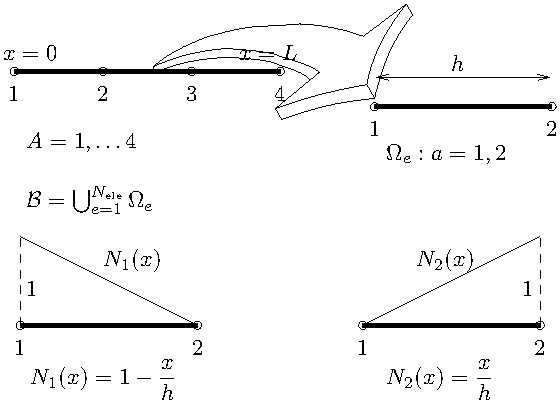
\includegraphics[width=0.55\textwidth]{figuras_1/FIG/malla1D-global-local-Nx.pdf}
\caption{Esquema de las funciones de forma lineales del elemento 2 de una discretización 1D de una barra con 3 elementos}
\label{fig:funciones_forma}
\end{figure}

Teniendo en cuenta los valores de $N_1$ y $N_2$ que aparecen en la figura~\ref{fig:funciones_forma}, se realizan las integrales de cada uno de los términos; por ejemplo $K_{11}^{e}$ es:
\begin{equation}
K_{11}^{e}=\int_{0}^{h} \frac{\mathrm{d} N_{1}}{\mathrm{d} x} EA \frac{\mathrm{d} N_{1}}{\mathrm{d} x} \mathrm{d} x=\frac{EA}{h^{2}} h=\frac{EA}{h}
\end{equation}\label{eq:N9}
y análogamente los demás:
\begin{equation}
K_{22}^{e}=\frac{EA}{h} ; \quad K_{12}^{EA}=K_{21}^{e}=-\frac{EA}{h}
\end{equation}\label{eq:N10}
resultando
\begin{equation}
\left[\mathbf{K}^{e}\right]=\frac{EA}{h}\left(\begin{array}{cc}{1} & {-1} \\ {-1} & {1}\end{array}\right)
\end{equation}\label{eq:N11}
Similarmente el vector de fuerzas internas del elemento resulta
\begin{equation}
\left\{\mathbf{f}^{\mathrm{int}, e}\right\}=\frac{h}{6}\left\{\begin{array}{l}{2q_1+q_2} \\ {q_1 + 2q_2}\end{array}\right\}
\end{equation}\label{eq:N12}

%Si considerásemos una carga repartida constante, dicho vector de fuerzas elemental se podría expresar como:
%\begin{equation}
%\left\{\mathbf{f}^{\mathrm{int}, e}\right\}=q h\left\{\begin{array}{l}{1 / 2} \\ {1 / 2}\end{array}\right\}
%\end{equation}\label{eq:N12_bis}

Una vez formadas las matrices elementales se convierten a
numeración global,
\begin{eqnarray}
K_{a b}^{e} & \rightarrow\left[\hat{\mathbf{K}}^{e}\right] \nonumber
 \\
f_{a}^{e} & \rightarrow \lbrace\hat{\mathbf{f}}^{e}\rbrace \nonumber
\end{eqnarray}
ensamblándose finalmente estas matrices locales dentro de las matrices globales del sistema. Para el ejemplo de la figura~\ref{fig:funciones_forma}, puesto que todos los elementos son iguales, las matrices elementales de rigidez son todas iguales entre sí, siendo su valor el de la matriz de la ecuación~\eqref{eq:N11}.

Para poder realizar el ensamblaje hay que tener en cuenta el lugar que van a ocupar en la matriz de rigidez global las distintas componentes de las matrices de rigidez locales. Si observamos la figura~\ref{fig:funciones_forma} vemos que el elemento 1 y el elemento 2 comparten el nodo número 2, por eso la posición $(2,2)$ de la matriz de rigidez global será compartida por las matrices de rigidez locales de los elementos 1 y 2. La forma que tendrá esta matriz de rigidez global será:

\begin{equation}
  K^{global} = \left[
  \begin{BMAT}[8pt]{cccc}{cccc}
   K_{11}^{(1)} & K_{12}^{(1)} & 0 & 0\\
   K_{21}^{(1)} & K_{22}^{(1)}  + K_{11}^{(2)} & K_{12}^{(2)} & 0 \\
    0 & K_{21}^{(2)} & K_{22}^{(2)} + K_{11}^{(3)}  & K_{12}^{(3)} \\
    0 & 0 & K_{21}^{(3)} & K_{22}^{(3)}
  \addpath{(0,4,.)rrddlluu}
  \addpath{(1,3,.)rrddlluu}
   \addpath{(2,2,.)rrddlluu}
  \end{BMAT}\right]
\end{equation}

De este ensamblaje, teniendo en cuenta los valores de las matrices de rigidez locales, obtenemos la matriz de rigidez global:
$$
[\mathbf{K}]=\frac{EA}{h}\left(\begin{array}{cccc}{1} & {-1} & {0} & {0} \\ {-1} & {1+1} & {-1} & {0} \\ {0} & {-1} & {1+1} & {-1} \\ {0} & {0} & {-1} & {1}\end{array}\right)
$$
Las matrices elementales y global de fuerzas internas son
$$\left\{\mathbf{f}^{\mathrm{int}, e}\right\}=\frac{h}{6}\left\{\begin{array}{l}{2q_1+q_2} \\ {q_1 + 2q_2}\end{array}\right\}
\Rightarrow\left\{\mathrm{f}^{\mathrm{int}}\right\}=\frac{h}{6}\left\{\begin{array}{c}{2q_1^{(1)}+q_2^{(1)}} \\ {q_1^{(1)} + 2q_2^{(1)} + 2q_1^{(2)}+q_2^{(2)}} \\ {q_1^{(2)} + 2q_2^{(2)} + 2q_1^{(3)}+q_2^{(3)}}  \\ {q_1^{(3)} + 2q_2^{(3)}}\end{array}\right\}
$$

Si considerasemos una restricción del movimiento en el extremo $x=0$ y una carga $q_L$ aplicada en el extremo $x=L$, la ecuación matricial que resulta de aplicar el método de los Elementos Finitos es:
$$
[\mathbf{K}]\{\mathbf{u}\}=\left\{\mathbf{f}^{\text {int }}\right\}+\left\{\mathbf{f}^{\text {ext }}\right\}
$$
\begin{equation}
\frac{EA}{h}\left(\begin{array}{c;{2pt/2pt}ccc}{1} & {-1} & {0} & {0} \\ 
\hdashline[2pt/2pt]
{-1} & {1+1} & {-1} & {0} \\ {0} & {-1} & {1+1} & {-1} \\ {0} & {0} & {-1} & {1}\end{array}\right)
\left\{\begin{array}{l}0\\
\hdashline[2pt/2pt]
u_2 \\ u_{3} \\ u_{4}\end{array}
\right\}=
\frac{h}{6}\left\{\begin{array}{c}{2q_1^{(1)}+q_2^{(1)}} \\ 
\hdashline[2pt/2pt]
{q_1^{(1)} + 2q_2^{(1)} + 2q_1^{(2)}+q_2^{(2)}} \\ {q_1^{(2)} + 2q_2^{(2)} + 2q_1^{(3)}+q_2^{(3)}}  \\ {q_1^{(3)} + 2q_2^{(3)}}\end{array}\right\}
+\left\{\begin{array}{c} R_0 \\
\hdashline[2pt/2pt]
{0} \\ {0} \\ {P}\end{array}\right\}
\end{equation}
 
Al vector de fuerzas volumétricas se le suma el de externas, en este caso una posible carga en P. Por otro lado, en el extremo $x=0$ existe una reacción para que el desplazamiento sea igual al impuesto, $u(0)=0$. Dicha reacción se calcula \textit{a posteriori,} una vez calculados los desplazamientos $\{\mathbf{u}\}$. \\
 
Una vez calculados los desplazamientos por la inversión de la matriz de rigidez, ya reducida por la aplicación de las condiciones de contorno, cabe la posibilidad de verificar el equilibrio, que se puede obtener como resultado de la suma de las fuerzas internas del cuerpo, que, en el caso del equilibrio, deben ser 0, siendo estas fuerzas internas calculadas como:
 $$
\left\{\mathbf{f}^{\text {int}}\right\}=[\mathbf{K}]\{\mathbf{u}\}
$$
 
 Por otro lado, la reacción en este caso se podría calcular multiplicando la fila eliminada de la matriz $[\mathbf{K}]$ por el vector de desplazamientos y restándole las fuerzas aplicadas en dicho nodo, que, al tratarse de un contorno tipo \emph{esencial}, solo podrán ser fuerzas volumétricas:
 $$
 R_0=K_{1j}u_j-f^{\text {vol}}_1
$$


\clearpage
\section{Tareas para entregar}
\label{sec:tareas}

Se desea calcular la respuesta de una fibra elástica unidimensional, de longitud \(L=10 \mathrm{mm}\)
y sección uniforme \(A=1 \mathrm{mm}^{2} .\) El material es elástico lineal, con módulo de Young \(E=1000 \mathrm{MPa}\).
El extremo izquierdo \((x=0)\) está fijo mientras que sobre el derecho \((x=L)\) actúa una fuerza
axial de valor \(P=5 \mathrm{N},\) como se indica en la figura~\ref{fig:esq}. Se podrá suponer que las deformaciones
son pequeñas.

\begin{figure}[!htp]
\centering
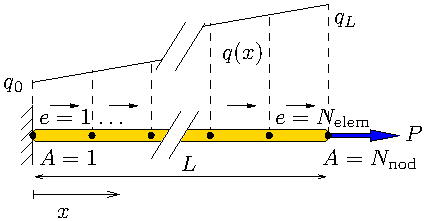
\includegraphics[width=0.7\textwidth]{figuras_1/esquema.pdf}
\caption{Modelo de fibra elástica 1D}
\label{fig:esq}
\end{figure}

A partir de los dígitos de las decenas (d) y unidades ( \(u\) ) del número de matricula de cada estudiante, \(N_{\text {mat }}=d u,\) se tomarán los siguientes parámetros para el modelo:
\begin{itemize}
\item Número de elementos \(N_{\text {elem }}=9-d\)
\item La carga distribuida \(q(x),\) fuerza longitudinal por unidad de longitud, será lineal entre los extremos \(x=0\) y \(x=L,\) con los valores en los extremos \(q_0=d / 10\; \mathrm{N} / \mathrm{mm}, \quad q_{L}=q_{0}+u / 10 \; \mathrm{N} / \mathrm{mm} \).
\end{itemize}

Los pasos a seguir son:
\begin{enumerate}
\item Planteamiento del problema elástico y condiciones de contorno.
\item Expresiones numéricas de las matrices de rigidez y de fuerzas del modelo completo.
\item Aplicación de condiciones de contorno y resolución.
\item Solución para los desplazamientos \(u(x)\) y tensiones \(\sigma(x)\) en cada punto, dibujando la gráfica en función de \(x\) y comparando con la solución analítica. (Nota: las tensiones se calculan
a partir de los desplazamientos como \(\sigma=E \varepsilon=E \mathrm{d} u / \mathrm{d} x,\) y empleando la aproximación
en un elemento finito, \(\left.\sigma^{h}=E u_{a} \mathrm{d} N_{a} / \mathrm{d} x=E\left(u_{2}-u_{1}\right) / h .\right)\)
\end{enumerate}

Se pide:
\begin{enumerate}
\item  Desarrollo de la solución analítica.
\item Comparativa de las soluciones analítica y numérica para los desplazamientos \(u(x)\) y las tensiones.
\item Discutir los resultados. ¿Qué forma tienen las tensiones? ¿Por qué?
\end{enumerate}

Se recomienda emplear \texttt{Matlab} como software de referencia.\\

Al finalizar la clase se debe entregar, en una tarea en \emph{Moodle}, un archivo  \texttt{*.m} donde se evaluará la capacidad de resolución del problema. NO ES OBLIGATORIO HABER ACABADO EL PROBLEMA.


Si no se ha acabado el \emph{script} de \texttt{MatLab} y respondidas a las cuestiones planteadas, se deberá completar en casa y ha de ser entregado en conjunto con la práctica 8.2, donde se resolverá el problema también con \texttt{FeBio}. Se habilitará una nueva tarea de \emph{Moodle} en el horario indicado, valorándose en este caso la discusión que se realice de los resultados.

\section{Organización del código }
\label{sec:esq}

La organización del código de \texttt{Matlab} es totalmente libre, pero, puesto que es la primera aproximación que el alumno hace a un código de elementos finitos, el seguir el esquema~\ref{codigo1} puede resultar muy interesante para seguir unas pautas.

\begin{lstlisting}[ label=codigo1,caption=Esquema Matlab]
% A: PREPROCESO
%----------------------------------------------------------------
% 1. Geometría

% 2. Material

% 3. Condiciones de contorno en carga

% 4. Malla

% 5. Grados de Libertad del problema


% B: CONSTRUCCIÓN de MATRICES y VECTORES globales
%----------------------------------------------------------------

% C: APLICACIÓN de las CONDICIONES de CONTORNO y RESOLUCIÓN
%----------------------------------------------------------------

% D: POSTPROCESO
%----------------------------------------------------------------


\end{lstlisting}


\clearpage
\section{Primeros pasos}
\label{sec:1pasos}

\begin{lstlisting}[ label=codigo2,caption=Primeros pasos]
% Definición de parámetros particulares de cada alumno
Nmat=24             % número de matrícula del alumno
d=floor(Nmat/10)    % cifra de decenas
u=Nmat-d*10         % cifra de unidades

% A: PREPROCESO
%----------------------------------------------------------------
% 1. Geometría
A=1;              % Area
L=10;             % Longitud de la fibra

% 2. Material
E=1000;           % datos del enunciado

% 3. Condiciones de contorno en carga
P=5;              % dato de fuerza aplicada en x=L
q0=--;        
qf=---;

% 4. Malla
Nele=; %Dato del problema!!!
Nnod=; %Numero de nodos. Piensa!
H=; %Tamaño de elemento, longitud entre numero de elementos
% Carga de cada nodo correspondiente a la carga repartida
q=----; % Que funcion conozco para hacer una distribucion lineal

% 5. Grados de Libertad del problema
% Dim = GDL totales = grados de libertad nodales x no nodos
gdl=1; % Desplazamiento en x
Dim=Nnod*gdl; 

% B: CONSTRUCCIÓN de MATRICES y VECTORES globales
%----------------------------------------------------------------
% 0. Inicialización
K=zeros(Dim); 
F=zeros(Dim,1); 
Fext=zeros(Dim,1);

% 1. Matriz de rigidez elemental (común a todos los elementos)
k=---;

% 2. Ensamblaje de la matriz global
for i=1:Nele
    ---
end

% 3. Ensamblaje del vector de fuerzas volumetricas global (diferente para cada elemento)
for i=1:Nele
    % vector elemental de cargas distribuidas
    f=---;
    % ensambla cargas
         ---             
end

% 4. Suma del vector de fuerzas externas
Fext(Nnod)=Fext(Nnod)+P;
F=F+Fext;           % suma cargas en contorno y cargas distribuidas


% C: APLICACIÓN de las CONDICIONES de CONTORNO y RESOLUCIÓN
%----------------------------------------------------------------

% 1. Reducción de la matriz de rigidez


% 2. Reducción del vector de fuerzas


% 3. Resuelve sistema reducido para desplazamientos
ug=Kg\Fg;  

% 4. Desplazamientos y reacciones. Equilibrio: Sum fuerzas = 0
un=[0;ug]; 
fint=------;
r_0=-----; 

Eq=sum(fint);
if ---- (Alcanzamos el equilibrio cuando las fuerzas internas suman 0... o casi 0....)
	disp('Equilibrio no alcanzado');
end

% D: POSTPROCESO
%----------------------------------------------------------------

% 1. Deformaciones y Tensiones
epsilon=zeros(Nele,1);
sigma=zeros(Nele,1);
for i=1:Nele
    epsilon(i)=----
    sigma(i)=---
end


% 2. Solución analítica
dx=20;
xc=linspace(0,L,dx);
dq=qf-q0;
r=dq/L; uc=1/(E*A)*((P+q0*L+1/2*r*L^2)*xc-(1/2*q0*xc.^2+1/6*r*xc.^3)); sigmac=1/A*(P+q0*(L-xc)+1/2*r*(L^2-xc.^2));

% 3. Gráfico
% 3.1. Dibuja la solucion del desplazamiento en x

% 3.2. Dibuja la solucion de la tensión en x


\end{lstlisting}